\documentclass[aspectratio=169]{beamer}
\mode<presentation>
%\usetheme{Warsaw}
%\usetheme{Goettingen}
\usetheme{Hannover}
%\useoutertheme{default}

%\useoutertheme{infolines}
\useoutertheme{sidebar}
\usecolortheme{dolphin}


\setbeamersize{sidebar width left=0pt} % to remove the sidebar
\beamertemplatenavigationsymbolsempty % To remove the navigation symbols on the bottom right.
\setbeamersize{text margin left=10mm,text margin right=10mm} % Specify margins

\usepackage{amsmath}
\usepackage{amssymb}
\usepackage{listings}
\usepackage{enumerate}
\usepackage{hyperref}
\hypersetup{
    colorlinks=true,
    linkcolor=blue,
    filecolor=magenta,      
    urlcolor=cyan,
}
\usepackage{tikz}  %For grpah drawing 
 
\urlstyle{same}

%some bold math symbosl
\newcommand{\Cov}{\mathrm{Cov}}
\newcommand{\Var}{\mathrm{Var}}
\newcommand{\brho}{\boldsymbol{\rho}}
\newcommand{\bSigma}{\boldsymbol{\Sigma}}
\newcommand{\btheta}{\boldsymbol{\theta}}
\newcommand{\bbeta}{\boldsymbol{\beta}}
\newcommand{\bmu}{\boldsymbol{\mu}}
\newcommand{\bW}{\mathbf{W}}
\newcommand{\one}{\mathbf{1}}
\newcommand{\bH}{\mathbf{H}}
\newcommand{\by}{\mathbf{y}}
\newcommand{\bolde}{\mathbf{e}}
\newcommand{\bx}{\mathbf{x}}

\newcommand{\cpp}[1]{\texttt{#1}}

%--------------------------------------------------
\providecommand{\abs}[1]{\lvert#1\rvert}
\providecommand{\norm}[1]{\lVert#1\rVert}
\providecommand{\Blue}[1]{\textcolor{blue}{#1}}
\providecommand{\Red}[1]{\textcolor{red}{#1}}  
\providecommand{\Purple}[1]{\textcolor{purple}{#1}} %for notations
\newcommand{\celsius}{\ensuremath{^\circ}C}
\newcommand\thfore{\mathord{\therefore}\,}
%------------------------------------------------------------------

\title{Lecture 1. Introduction to Graph Theory}
\author{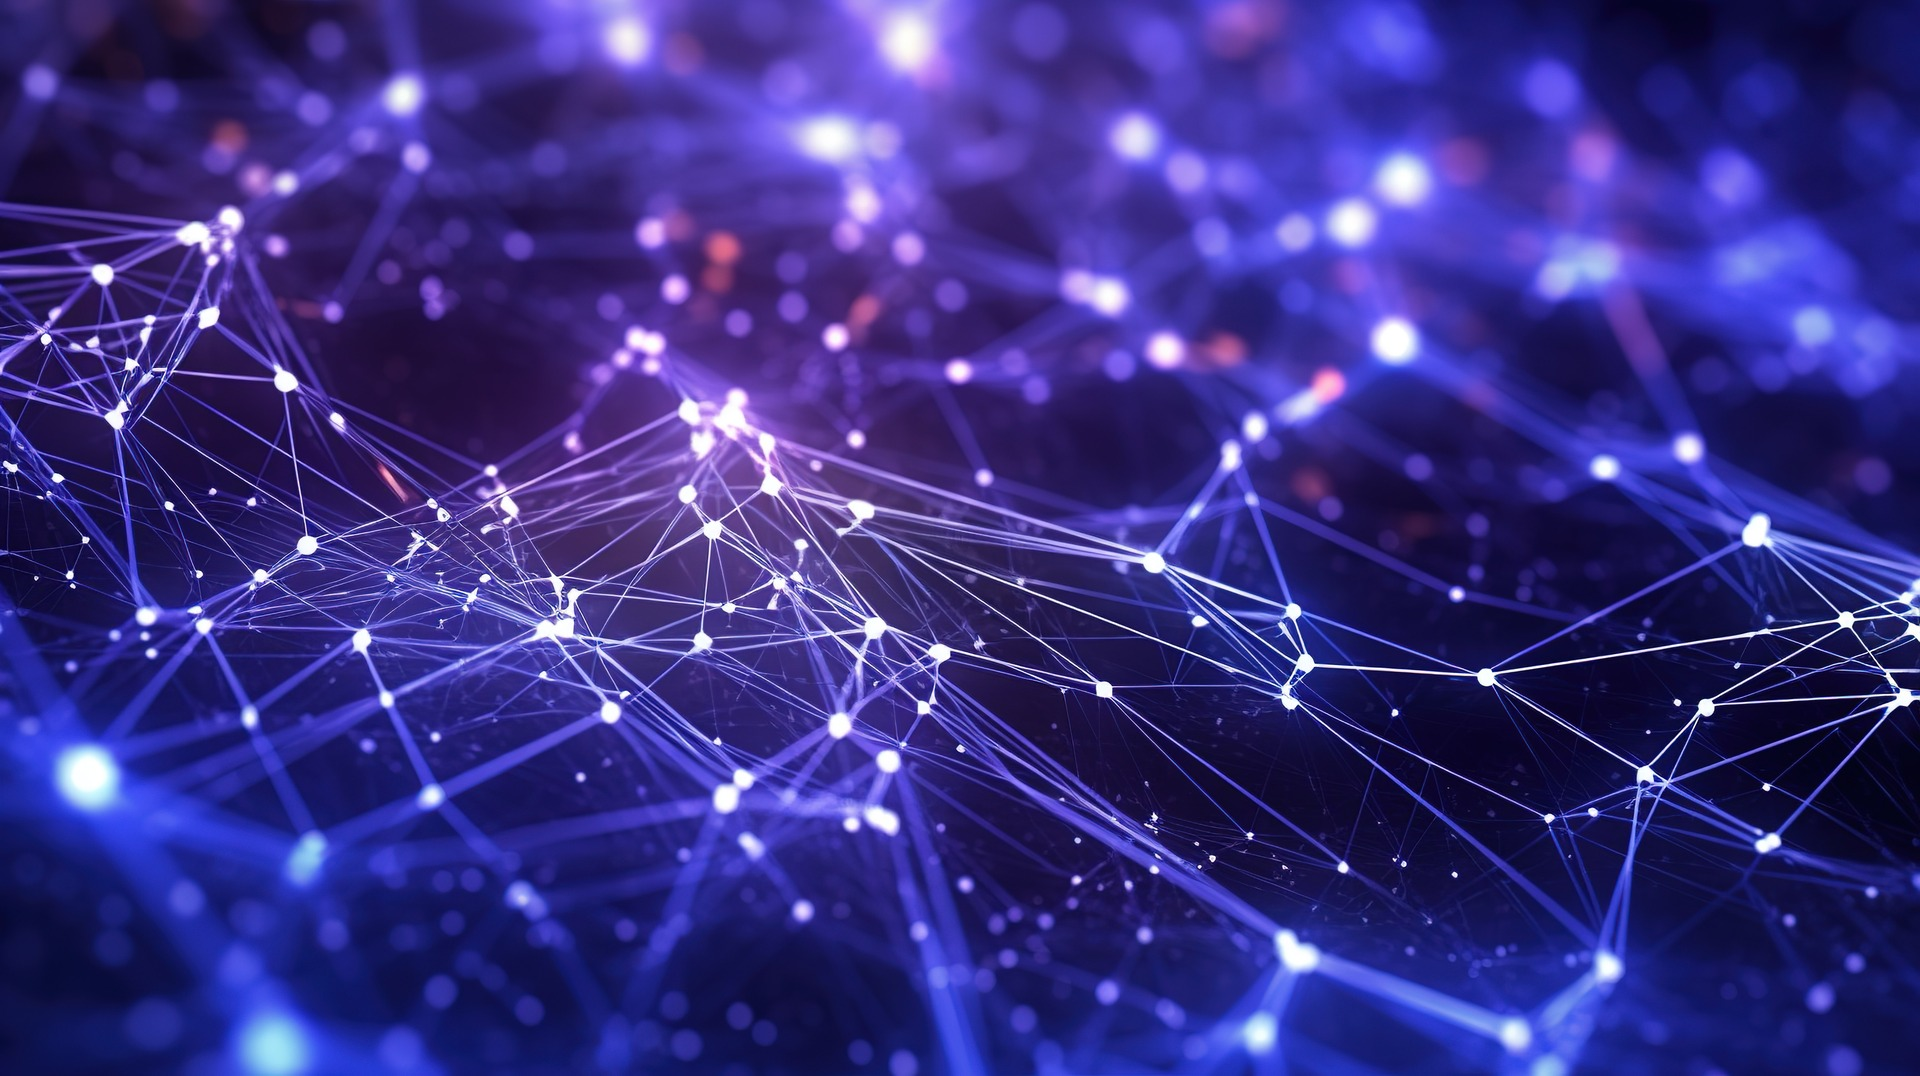
\includegraphics[width=.8\textwidth,height=.7\textheight]{./img/lecture1-fig0.jpeg}}
%Picture from   https://beta.yourengineer.in/article/what-is-a-neural-network-29e5

\date{ }
%------------------------------------------------------------------


\begin{document}

\frame[plain]{\titlepage}

\begin{frame}[plain]{What is a graph?} 

A \Blue{graph} is a structure consisting of 
  \Blue{vertices} (or \Blue{nodes}: points in the graph) and   \Blue{edges} (connections between pairs of vertices.)

 \vspace*{-1.0cm} 

\begin{figure}
\centering

\begin{columns}[t,onlytextwidth]
\column{.33\textwidth}
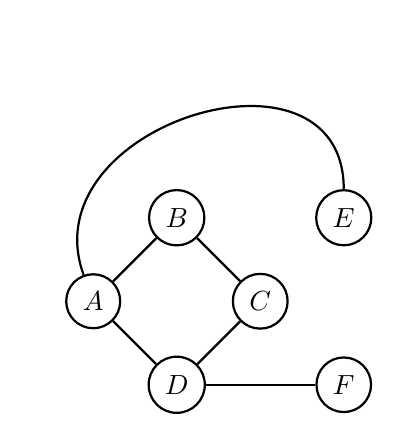
\begin{tikzpicture}[node distance={15mm}, thick, main/.style = {draw, circle}] 
\node[main] (1) {$A$}; 
\node[main] (2) [above right of=1] {$B$};
\node[main] (3) [below right of=1] {$D$}; 
\node[main] (4) [above right of=3] {$C$};
\node[main] (5) [above right of=4] {$E$}; 
\node[main] (6) [below right of=4] {$F$};

\draw (2) -- (4);
\draw (1) -- (2);
\draw (1) -- (3);
\draw (3) -- (4);
\draw (3) -- (6);
\draw (1) to [out=110,in=90,looseness=1.5] (5);
\end{tikzpicture} 

\smallskip

\begin{center}
 \Blue{(Undirected) Graph}
\end{center}

\column{.33\textwidth}
 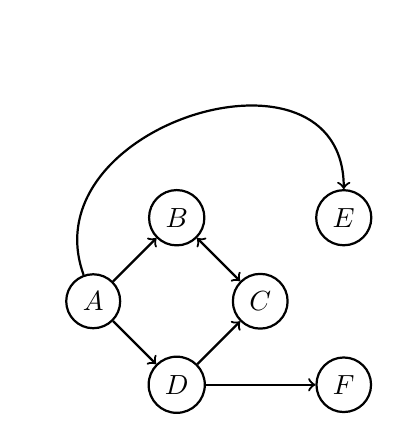
\begin{tikzpicture}[node distance={15mm}, thick, main/.style = {draw, circle}] 
\node[main] (1) {$A$}; 
\node[main] (2) [above right of=1] {$B$};
\node[main] (3) [below right of=1] {$D$}; 
\node[main] (4) [above right of=3] {$C$};
\node[main] (5) [above right of=4] {$E$}; 
\node[main] (6) [below right of=4] {$F$};

\draw[<->] (2) -- (4);
\draw[->] (1) -- (2);
\draw[->] (1) -- (3);
\draw[->] (3) -- (4);
\draw[->] (3) -- (6);
\draw[->] (1) to [out=110,in=90,looseness=1.5] (5);
\end{tikzpicture}
\smallskip

\begin{center}
 \Blue{Directed Graph}
\end{center}

\column{.33\textwidth}
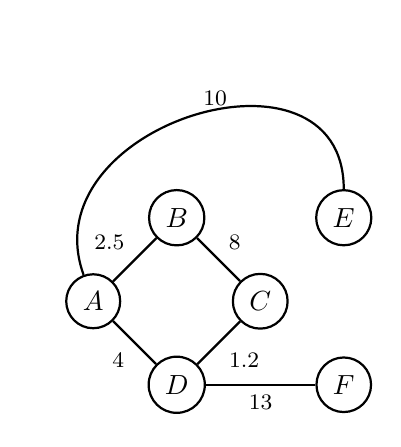
\begin{tikzpicture}[node distance={15mm}, thick, main/.style = {draw, circle}] 
\node[main] (1) {$A$}; 
\node[main] (2) [above right of=1] {$B$};
\node[main] (3) [below right of=1] {$D$}; 
\node[main] (4) [above right of=3] {$C$};
\node[main] (5) [above right of=4] {$E$}; 
\node[main] (6) [below right of=4] {$F$};

\draw (2) -- node[above right] {\footnotesize $8$} (4);
\draw (1) -- node[above left] {\footnotesize $2.5$}(2);
\draw (1) -- node[below left] {\footnotesize $4$} (3);
\draw (3) -- node[below right] {\footnotesize $1.2$} (4);
\draw (3) -- node[below ] {\footnotesize $13$} (6);
\draw (1) to [out=110,in=90,looseness=1.5] node[above right] 
       {\footnotesize $10$} (5);
\end{tikzpicture} 
\smallskip

\begin{center}
 \Blue{Weighted Graph}
\end{center}

\end{columns}

\end{figure}

\medskip

The vertices and edges of a graph might represent any number of different things, depending on the
application


\end{frame}


\begin{frame}[plain]{Applications of Graph Models}

{\bf Example 1.1.  Football Passing Networks}

  \begin{center}
	      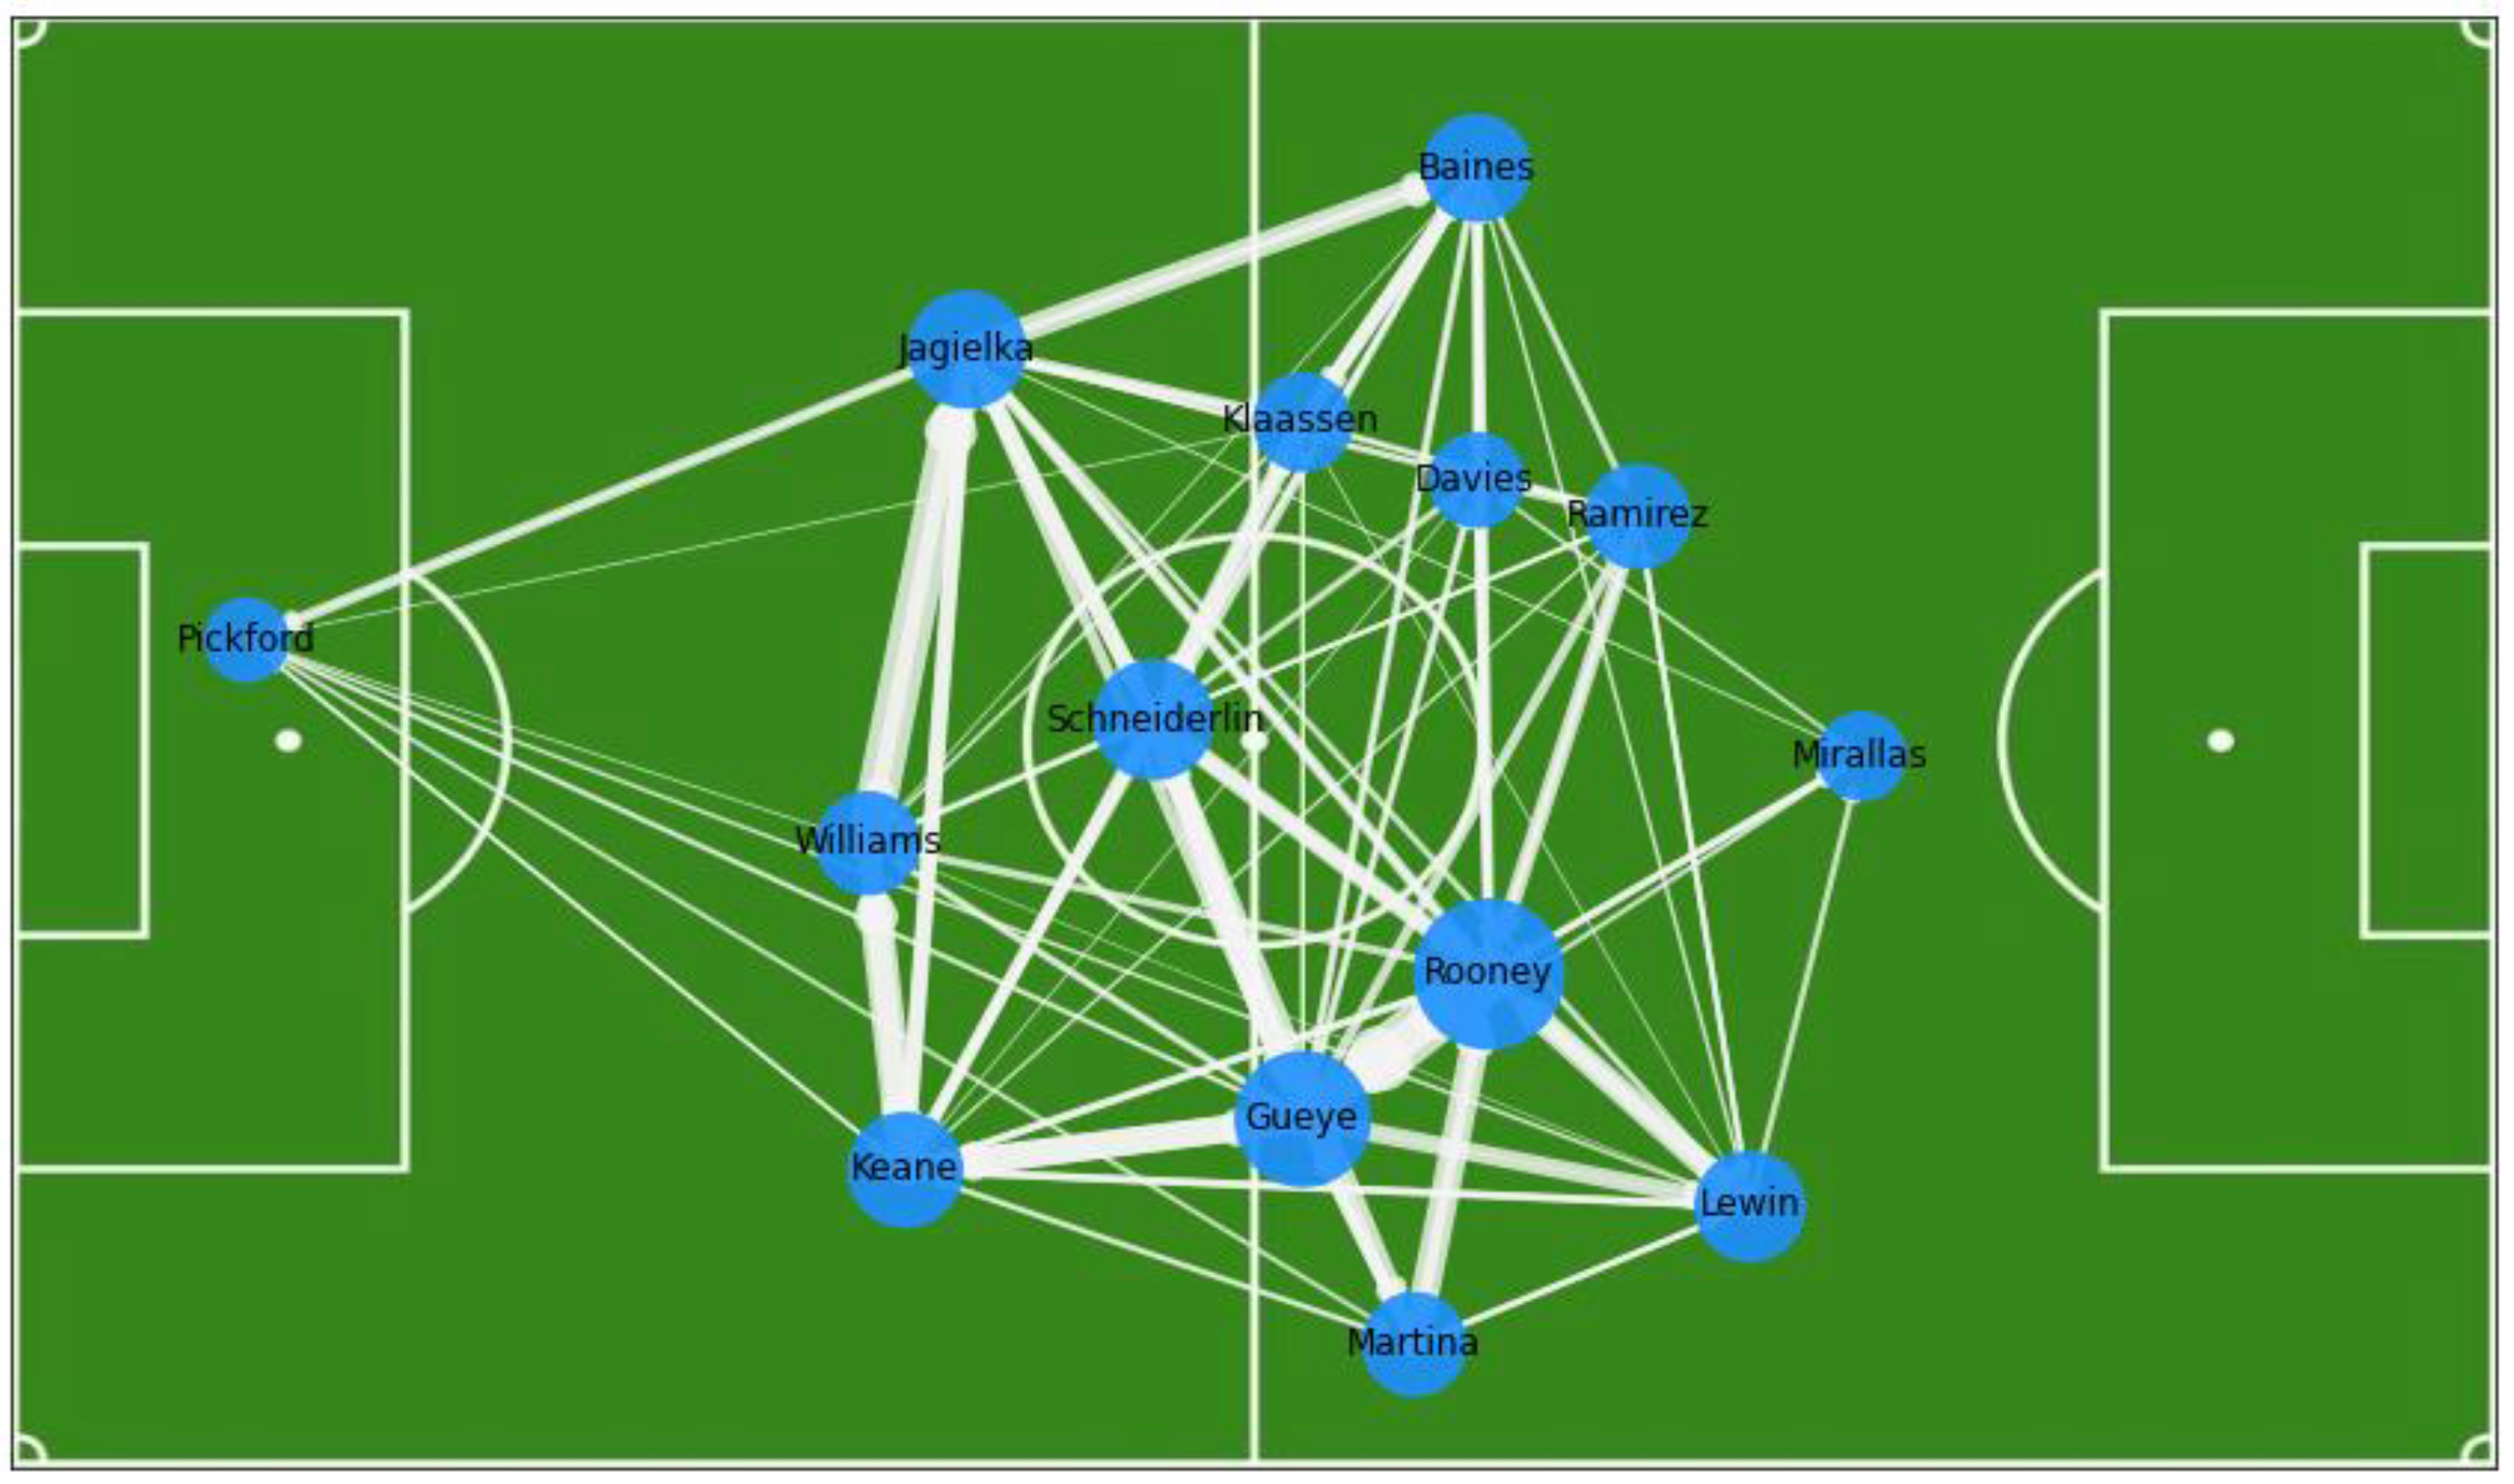
\includegraphics[height=6cm]{./img/lecture1-fig1.png}
  \end{center}

\end{frame}	

\begin{frame}[plain]{ }

{\bf Example 1.2}. %Source. https://beta.yourengineer.in/article/what-is-a-neural-network-29e5
A  \Blue{neural network} is a computational model inspired by the structure and functioning of the human brain. 
 It is widely used in machine learning tasks, such as image recognition, language processing, and data classification.
 
 \begin{center}
	      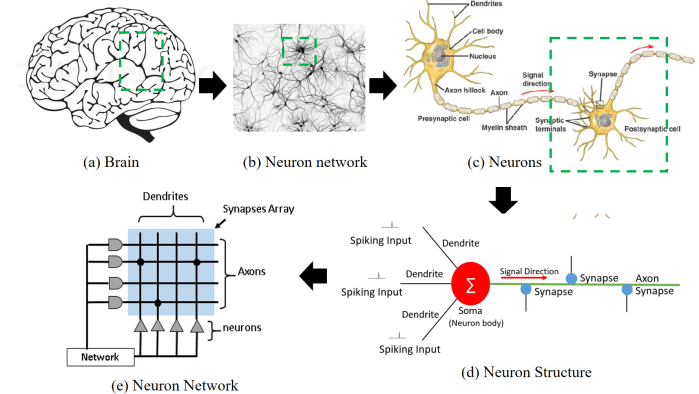
\includegraphics[height=6.5cm]{./img/lecture1-fig1-NN.png}
  \end{center}
	    
\end{frame}

\begin{frame}[plain]{}

A neural network can be modeled as a directed graph, where:
\begin{itemize}
	\item {\bf Vertices} represent \Blue{neurons}.
	\item {\bf Edges} represent connections (\Blue{synapses}) between neurons, carrying weights to define the strength of the connections.
\end{itemize}
\medskip

{\bf Structure of Neural Networks}:
  \begin{enumerate}
	\item 	Input Layer: The first layer, where data enters the network.
	\item 	Hidden Layers: Intermediate layers that process the data by performing weighted calculations and applying activation functions.
	\item 	Output Layer: The final layer that produces predictions or classifications.
 \end{enumerate}
 
{\bf Information Flow in Neural Networks}:
Data flows from the input layer through the hidden layers and finally to the output layer. 
Each connection has a weight and can be adjusted during training to optimize performance.

\end{frame}

\begin{frame}[plain]{}

Fully connected feed-forward neural network (perceptron):

	\begin{center}
	      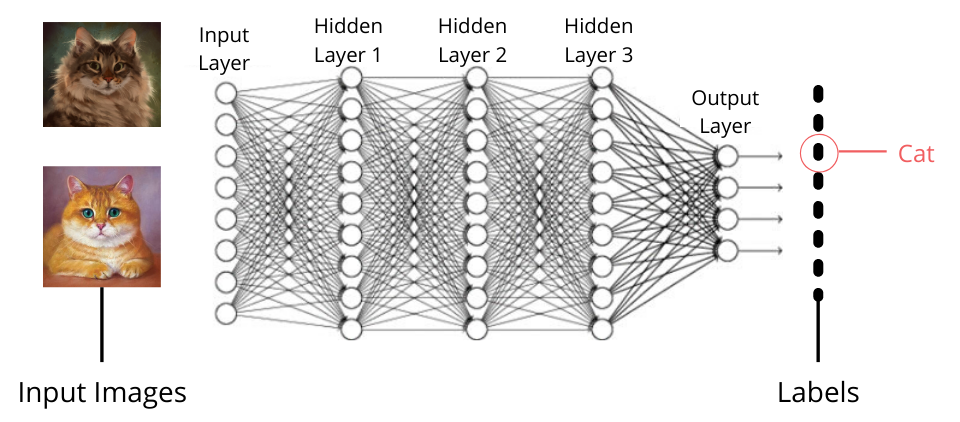
\includegraphics[height=6cm]{./img/lecture1-fig2.png}
	    \end{center}

\end{frame}

\begin{frame}[plain]{}

{\bf Problem 1.3}.  Model a feed-forward neural network as a directed weighted graph with the following details:

  \begin{itemize}
   \item Input Layer: 2 neurons labeled  $I_1$  and  $I_2 $.
   \item Hidden Layer: 3 neurons labeled  $H_1, H_2, H_3 $.
   \item Output Layer: 1 neuron labeled  $O_1$.
   \end{itemize}
   
   Graph Construction:
   \begin{enumerate}
     \item Draw vertices for each neuron.
     \item Add directed edges to represent connections:
        \begin{itemize}
	  \item Each input neuron connects to every hidden neuron.
	  \item Each hidden neuron connects to the output neuron.
       \end{itemize}
     \item Assign weights to the edges (use arbitrary values).  
   \end{enumerate}
   \vspace{.5in}
   
 \end{frame}


\begin{frame}[plain]{}

{\bf Exercise 1.4}. 
A  \Blue{ precedence graph} is a directed graph used in programming to represent the execution order of statements based on dependencies.

  \begin{itemize}
   \item Vertices: Represent program statements.
   \item Edges: A directed edge from vertex  $u$  to vertex $ v$  means that statement  $v$  cannot be executed until statement  $u$  has been executed.
 \end{itemize}
 
 Given the following statements and dependencies, draw a precedence graph. (Here, $S_1, S_2, ...$, are the order of computation process.)
 \medskip
 
 %	    \begin{center}
	\hspace{.2in}     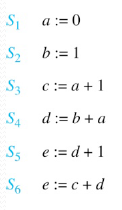
\includegraphics[height=3.3cm]{./img/lecture1-fig3a.png} % solution picture is  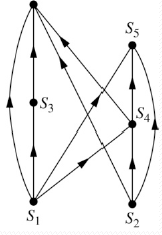
\includegraphics[height=3.3cm]{lecture1-fig3b.png}
%	    \end{center}


\end{frame}

\end{document}

